\paragraph{a)}
We have 52 observations contained in the domain $\mathcal{D} = (0,315)\times(0,315)$. In Figure \ref{fig:terrain2a} we see a non-stationary RF, based on the fact that the mean changes with the position of reference. 

\begin{figure}[htb]
    \centering
    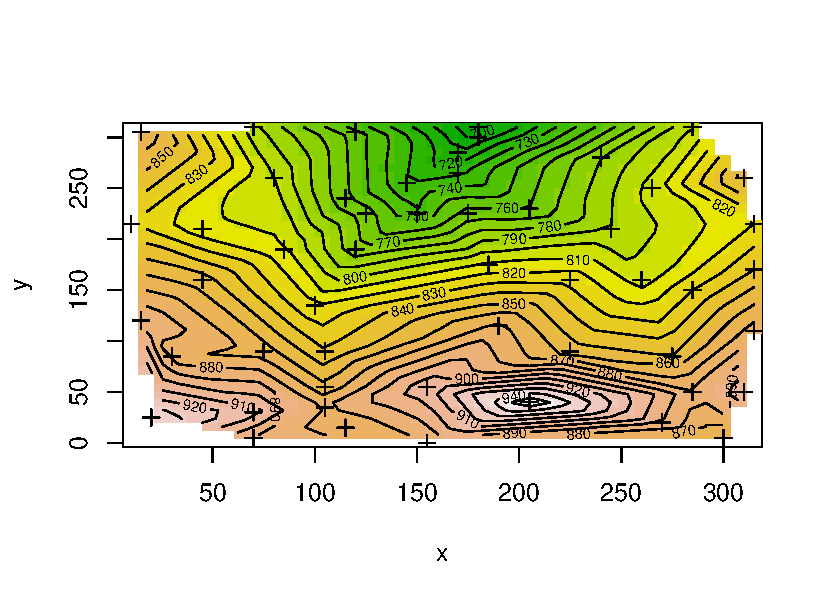
\includegraphics{figures/terrain2a.pdf}
    \caption{Contour plot with a heat-map of the interpolated observed data in $\mathcal{D}$}
    \label{fig:terrain2a}
\end{figure}


%%%%%%%%%%%%%%%%%%%%%%%%%%%%%%%%%%%%%%%%%%%%%%%%%%%%%%%%%%%%%%%%%%%%%%
\paragraph{b)}
Consider the continuous spatial variables $\{r(\vect{x}); \vect{x} \in \mathcal{D} \subset \mathbb{R}^2\}$ s.t.
\begin{equation}
\begin{array}{rcl}
     E[r(\vect{x})] & = & \vect{g}(\vect{x})^T\vect{\beta}_r \\
     \Var\{r(\vect{x})\} & = & \sigma_r^2 \\
     \Corr\{r(\vect{x}),r(\vect{x}^{'})\} & = & \rho_r(\vect{\tau}/\xi)
\end{array}
\end{equation}
with $\vect{g}(\vect{x}) = (g_1(\vect{x}), ... g_{n_g}(\vect{x}))$ a vector of known spatial variables and $\beta_r = (\beta_1, ..., \beta_{n_g})$ an unknown parameter. $\sigma_r^2 = 2500$ and the spatial correlation function have $\xi = 100$ with $\tau = |\vect{x} - \vect{x^{'}}|$. The prediction is 
\begin{equation}
    \hat{r}_0 = \vect{\alpha}^T\vect{r}_{n_g},
\end{equation}
with $\vect{\alpha} = (\alpha_1, ..., \alpha_{n_g})$ being the weights. 
The predictor error needs to be unbiased, which mean that the expected value of the error must be zero, giving
\begin{equation*}
\begin{array}{rcl}
    \E[\hat{r}_0 - r_0] & = & \vect{\alpha}^T \E[r^g]\\
      & \Downarrow & \\
      \vect{\alpha}^T \matr{G}_g \beta_r^+ & = & \vect{g}(\vect{x}_0) \\
      & \Downarrow & \\
      \matr{G}_g^T \vect{\alpha} & = & \vect{g}(\vect{x}_0)
\end{array}
\end{equation*}
with the ($n_g x n_g$)-matrix $\matr{G}_g = (\vect{g}(\vect{x}_1,...,\vect{g}(\vect{x}_{n_g})^T$.
The optimization problem comes from minimizing the prediction error variance. It is derived from
\begin{equation*}
    \begin{array}{rcl}
        \vect{\hat{\alpha}} & = & \arg\min\limits_\alpha \Var\{\hat{r}_0 - r_0\} \\
         & = & \arg\min\limits_\alpha\{\sigma_r^2 - 2\vect{\alpha}^T\sigma_r^2\vect{\rho}_0 + \vect{\alpha}^T\sigma_r^2\matr{\Sigma}_g^\rho \vect{\alpha}\} \\
          & \textrm{constrained by} & \matr{G}_g^T \vect{\alpha} = \vect{g}(\vect{x}_0)
    \end{array}
\end{equation*}
The analytical solution using optimization with lagrange multipliers is
\begin{equation*}
    \vect{\hat{\alpha}} = [\matr{\Sigma}_g^\rho]^{-1}\left[\vect{\rho}_0 - \matr{G}_g^T [\matr{G}_g[\matr{\Sigma}_g^\rho]^{-1}\matr{G}_g^T]^{-1}[\matr{G}_g[\matr{\Sigma}_g^\rho]^{-1}\vect{\rho}_0 - \vect{g}(\vect{x}_0)]\right]
\end{equation*}
which yields the universal kriging predictor and the associated prediction variance at an
arbitrary location $\vect{x}_0 \in \mathcal{D}$.
\begin{equation}
    \begin{array}{rcl}
         \hat{r}_0 & = & \vect{\hat{\alpha}}^T \vect{r}_{n_g}  \\
         \sigma_{\hat{r}}^2 & = & \sigma_r^2\left[1-2\vect{\hat{\alpha}}^T \vect{\rho}_0 + \vect{\hat{\alpha}}^T\matr{\Sigma}_g^\rho \vect{\hat{\alpha}}\right] 
    \end{array}
\end{equation}
%%%%%%%%%%%%%%%%%%%%%%%%%%%%%%%%%%%%%%%%%%%%%%%%%%%%%%%%%%%%%%%%%%%%%%
\paragraph{c)}
Let the reference variable $\vect{x} \in \mathcal{D} \subset \mathbb{R}^2$ be $\vect{x} = (x_v, x_h)$ with $n_g = 6$, and $\vect{g}(\vect{x})$ is $x_v^kx_h^l$ for $(k,l) \in \{(0,0),(1,0),(0,1),(1,1),(2,0),(0,2)\}$. Which means that the $n_g$-vector $\vect{g}(\vect{x}) = (1,x_v,x_h,x_vx_h,x_v^2,x_h^2)^T$. Looking at the expected value for $r(\vect{x})$ we get
\begin{equation*}
    \E[r(\vect{x})] = \vect{g}(\vect{x})^T \vect{\beta}_r = \beta_r^1 + x_v \beta_r^2 + x_h \beta_r^3 + x_v x_h \beta_r^4 + x_v^2 \beta_r^5 + x_h^2 \beta_r^6.
\end{equation*}
The values of $\vect{\beta}_r$ is unknown, but we don't need them to find the prediction. This is because of the unbiasedness of the expectation of the error in the prediction. 
The expected value does not include the variance, and the variance does not involve the actually values of the observations. 
In Figure \ref{fig:uk2} we see a heat map with contours of the predicted values $\hat{r}_{\vect{x}_0}$ and it looks familiar to what we got in the interpolation made in Figure \ref{fig:terrain2a}. In Figure \ref{fig:uk2se} we see the variance in the prediction, and we see that the values are low close to the observed values and higher far away from them. Which is what we should expect from the model.
\begin{figure}[htb]
    \centering
    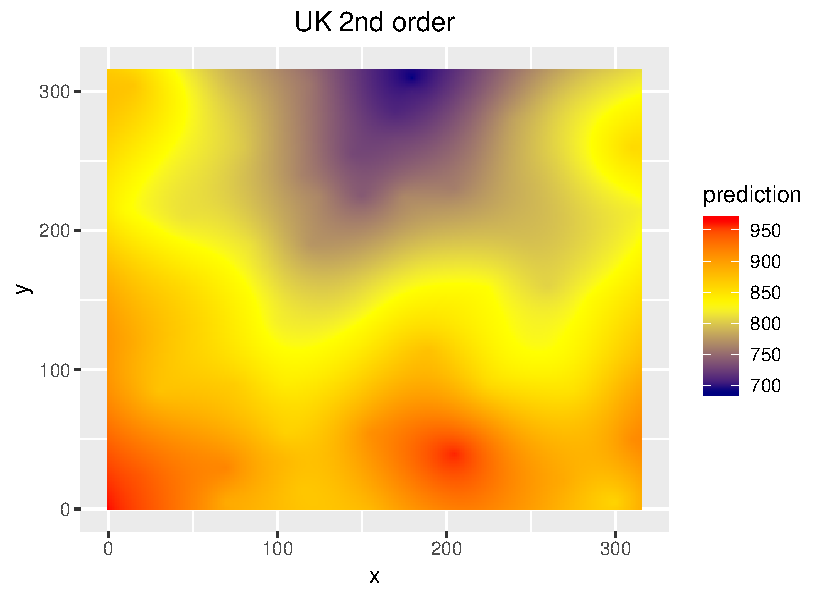
\includegraphics{figures/uk2.pdf}
    \caption{Heat-map of the predicted value $\hat{r}_{\vect{x}_0}$ on a grid $(0,315)\times(0,315)$ with second order expectation function.}
    \label{fig:uk2}
\end{figure}

\begin{figure}[htb]
    \centering
    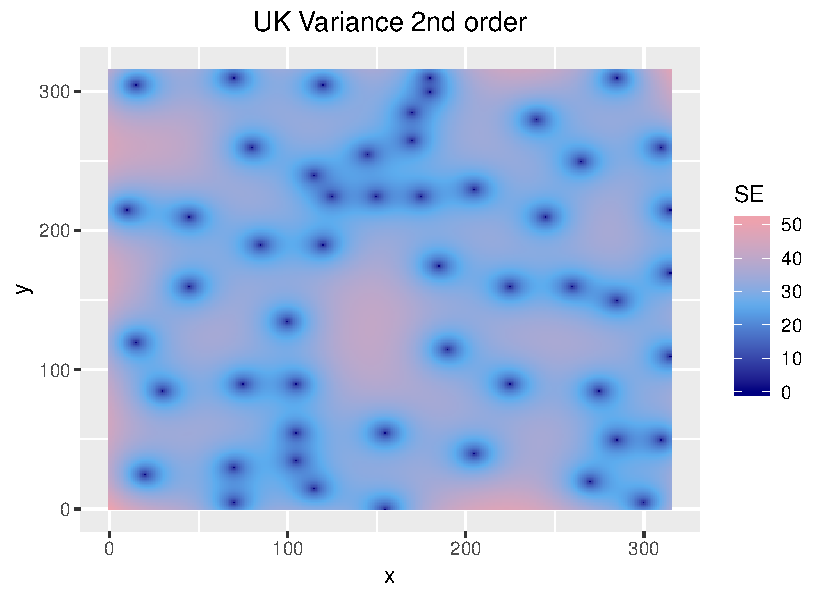
\includegraphics{figures/uk2se.pdf}
    \caption{Heat-map of the predicted variance $\sigma_{\hat{r}_{\vect{x}_0}}$ on a grid $(0,315)\times(0,315)$ with second order expectation function.}
    \label{fig:uk2se}
\end{figure}

\begin{figure}[htb]
    \centering
    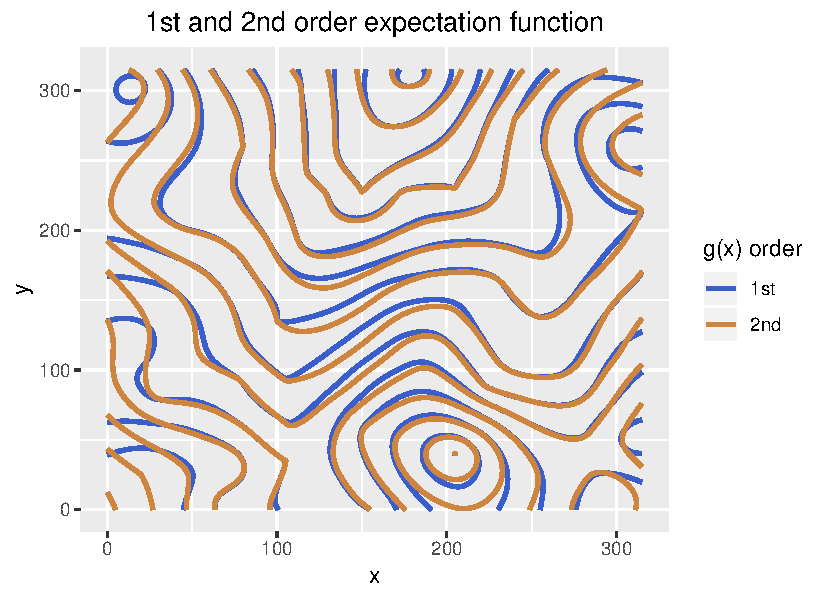
\includegraphics{figures/uk1n2.pdf}
    \caption{Heat-map of the predicted variance $\sigma_{\hat{r}_{\vect{x}_0}}$ on a grid $(0,315)\times(0,315)$ with second order expectation function.}
    \label{fig:uk1n2}
\end{figure}

%%%%%%%%%%%%%%%%%%%%%%%%%%%%%%%%%%%%%%%%%%%%%%%%%%%%%%%%%%%%%%%%%%%%%%
\paragraph{d)}
The probability for the height to be higher than 700 at the point $\vect{x}_0 = (100,100)$ is a normal distribution. In Figure \ref{fig:uk2} the points around $\vect{x}_0$ is around 850. The calculation yields 
\begin{equation*}
    P\left(Z>\frac{700 - \hat{r}_{\vect{x}_0}}{\sigma_{\hat{r}_{\vect{x}_0}}}\right) = 1-P\left(Z\leq\frac{700 - \hat{r}_0}{\sigma_{\hat{r}_{\vect{x}_0}}}\right) = 1.
\end{equation*}
So the probability for the height to be higher than 700 in $\vect{x}_0$ is 100\%.
The height at which the probability is 0.90 of the true height being lower than the predicted height at $\vect{x}_0$ is
\begin{equation*}
    Z|_{P = 0.9} = \frac{alt - \hat{r}_{\vect{x}_0}}{\sigma_{\hat{r}_{\vect{x}_0}}} = 1.28 \Rightarrow alt = 
\end{equation*}


%%%%%%%%%%%%%%%%%%%%%%%%%%%%%%%%%%%%%%%%%%%%%%%%%%%%%%%%%%%%%%%%%%%%%%
\paragraph{e)}
\begin{figure}[htb]
    \centering
    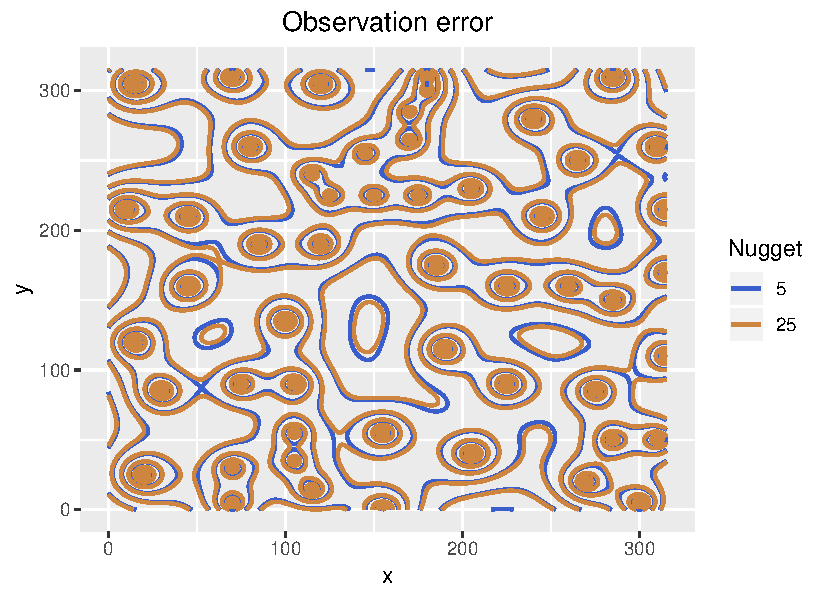
\includegraphics{figures/nugget.pdf}
    \caption{Heat-map of the predicted variance $\sigma_{\hat{r}_{\vect{x}_0}}$ on a grid $(0,315)x(0,315)$ with second order expectation fucntion.}
    \label{fig:nugget}
\end{figure}
%%%%%%%%%%%%%%%%%%%%%%%%%%%%%%%%%%%%%%%%%%%%%%%%%%%%%%%%%%%%%%%%%%%%%%
\paragraph{f)}
text text text
+